% Build from the repository root:
%   latexmk -pdf -outdir=/tmp/dd2482-report report.tex
% Replace the author field before submission.
% Sections 7 and 8 are intentionally reserved for the project authors.
\documentclass[10pt,a4paper]{article}
\usepackage[T1]{fontenc}
\usepackage[utf8]{inputenc}
\usepackage{lmodern}
\usepackage[margin=17mm]{geometry}
\usepackage{microtype}
\usepackage[hidelinks]{hyperref}
\usepackage{titlesec}
\usepackage{tikz}
\usetikzlibrary{arrows.meta,positioning,fit,backgrounds}
\titleformat{\section}{\large\bfseries}{\thesection}{0.6em}{}
\titlespacing*{\section}{0pt}{10pt}{5pt}
\setlength{\parindent}{0pt}
\setlength{\parskip}{5pt}
\newcommand{\file}[1]{\texttt{\nolinkurl{#1}}}
\newcommand{\reportauthors}{[Names and KTH IDs]}
\hypersetup{pdftitle={Snip: An Integrated DevOps Pipeline},pdfauthor={DD2482 project team}}
\begin{document}
\begin{center}
  {\LARGE\bfseries Snip: An Integrated DevOps Pipeline}\\[5pt]
  {DD2482 Project Report \enspace---\enspace \reportauthors}\\[3pt]
  {8 October 2026 \enspace\textbullet\enspace Repository snapshot: \texttt{8ac2f53}}
\end{center}

\section{Overview}
Snip is a URL shortener with a FastAPI backend, a dependency-free HTML/CSS/JavaScript frontend, and a SQLAlchemy persistence layer. 
Users create short links, follow redirects, inspect redirect counts, and disable links while retaining statistics. 
Although the application is small, its durable data and schema migrations make it suitable for demonstrating a complete DevOps workflow, from reviewed source changes to a verified deployment.

\begin{figure}[h!]
\centering
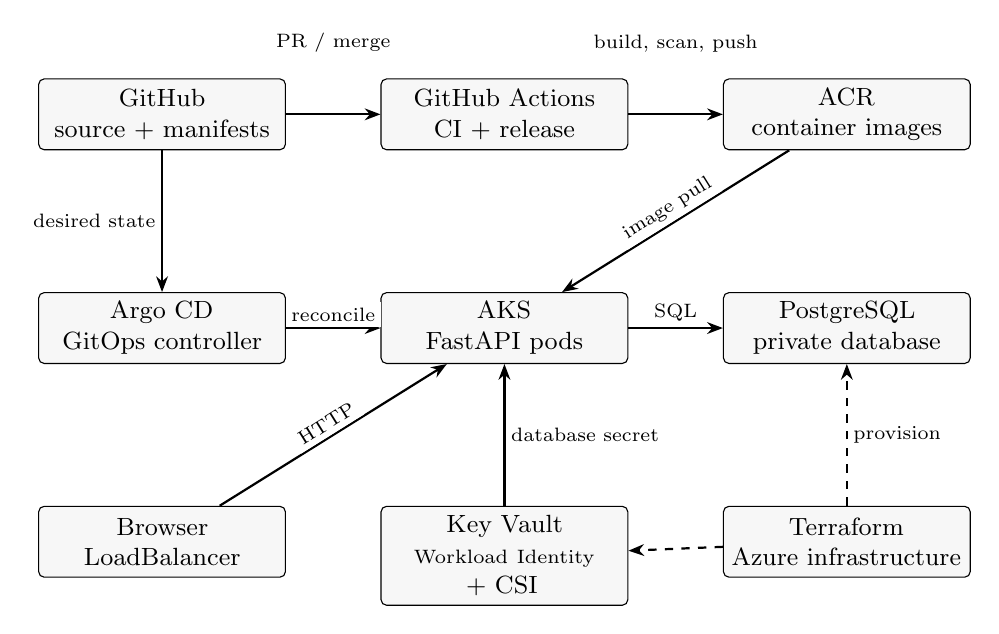
\begin{tikzpicture}[
  box/.style={draw,rounded corners=2pt,fill=black!3,align=center,font=\small,minimum height=9mm,text width=29mm},
  flow/.style={-{Stealth[length=2mm]},thick},
  note/.style={font=\scriptsize,align=center,fill=white,inner sep=2pt},
  node distance=11mm and 12mm
]
\node[box] (git) {GitHub\\source + manifests};
\node[box,right=of git] (ci) {GitHub Actions\\CI + release};
\node[box,right=of ci] (acr) {ACR\\container images};
\node[box,below=18mm of git] (argo) {Argo CD\\GitOps controller};
\node[box,right=of argo] (aks) {AKS\\FastAPI pods};
\node[box,right=of aks] (pg) {PostgreSQL\\private database};
\node[box,below=18mm of argo] (browser) {Browser\\LoadBalancer};
\node[box,below=18mm of aks] (kv) {Key Vault\\{\scriptsize Workload Identity}\\+ CSI};
\node[box,below=18mm of pg] (tf) {Terraform\\Azure infrastructure};
\draw[flow] (git) -- node[note,above=7mm]{PR / merge} (ci);
\draw[flow] (ci) -- node[note,above=7mm]{build, scan, push} (acr);
\draw[flow] (git) -- node[note,left]{desired state} (argo);
\draw[flow] (argo) -- node[note,above]{reconcile} (aks);
\draw[flow] (acr) -- node[note,sloped,above]{image pull} (aks);
\draw[flow] (aks) -- node[note,above]{SQL} (pg);
\draw[flow] (browser) -- node[note,sloped,above]{HTTP} (aks);
\draw[flow] (kv) -- node[note,right]{database secret} (aks);
\draw[flow,dashed] (tf) -- node[note,right]{provision} (pg);
\draw[flow,dashed] (tf) -- (kv);
\end{tikzpicture}
\caption{Delivery and runtime architecture. The release workflow also commits the selected image SHA back to GitHub. Terraform provisions AKS, ACR, networking, PostgreSQL, and Key Vault; dashed arrows illustrate provisioning.}
\end{figure}

The whole application was deployed onto Azure platform thanks to the free credits given to student accounts through KTH email.
The backend serves the API and frontend from one container, simplifying deployment. 
Azure Kubernetes Service (AKS) runs the pods, Azure Container Registry (ACR) stores images, and managed PostgreSQL 16 holds data outside the cluster.
A public LoadBalancer routes browser requests to the application. 
PostgreSQL has public access disabled and is reached through a delegated subnet and private DNS. 
Key Vault supplies the database connection through Azure Workload Identity and the Secrets Store CSI driver.

\section{CI pipeline}
Pull requests trigger a reusable GitHub Actions workflows for application quality, security, and configuration validation. 
The workflow installs Python 3.12 and uses \texttt{uv sync --locked} to reproduce dependencies from \file{uv.lock}. 
It runs Ruff formatting and lint checks, \texttt{ty} type checking, and tests through pytest.
The security workflow also builds the Docker image, making container build failures visible before a merge in order to understand earlier what could happen in production.

Unit tests check short-code generation. 
Integration tests cover API behavior, migrations, persistence across sessions, code-collision recovery, and redirect-counter updates from stale sessions.
These tests use SQLite, which keeps CI as quick as possible but leaves PostgreSQL-specific behavior untested.
The exact source commit on \texttt{main} passes the same quality, security, and configuration workflows again before release. 
This connects CI results to the source used to build the delivered image.

\newpage
\section{CD pipeline}
A push to \texttt{main} starts the CD workflow contained in \file{.github/workflows/release.yml}. 
After all validation jobs succeed(the ones mentioned before in the CI), the release job authenticates to Azure with OIDC, 
builds a source-SHA-tagged image, scans it, and pushes that same image to ACR.

A dedicated GitHub App obtains a temporary installation token and commits the image tag and \file{GIT_SHA} to the production Kustomize overlay. 
This Git commit records the selected application version for Argo CD.

Release jobs are serialized. 

A current-head check rejects already-stale source commits, and a normal push fails if \texttt{main} advances rather than overwriting newer changes. 
Pushes changing only the production overlay skip the release workflow, preventing release loops and allowing an existing image to be selected for rollback. 

SHA tags improve traceability, although digest pinning and registry-enforced immutability are not configured.
The mutable base image and OS package updates also mean rebuilding a source SHA may produce different image bytes.

Argo CD watches \texttt{main} at \file{k8s/overlays/production}. Automatic synchronization, pruning, and self-healing reconcile Kubernetes with Git. Namespace, ServiceAccount, and SecretProviderClass are applied at sync waves $-3$ and $-2$. The migration Job is a \texttt{Sync} hook at wave $-1$: it runs \texttt{alembic upgrade head} before the default-wave Deployment. A failed migration prevents the later rollout wave from proceeding.

The production overlay specifies two replicas and a rolling update with one surge pod and zero unavailable pods.
Liveness checks process availability; readiness queries the database and removes unready pods from Service traffic. 
Once the deployment is healthy, a \texttt{PostSync} Job creates a link, checks its HTTP 307 redirect destination, and disables it. 
Hook failures are visible in Argo CD but do not automatically revert the application. 
Actions finishes after publishing and committing desired state, so delivery success and deployment success are observed separately.
Reverting the overlay can select an earlier image, but does not undo database migrations. Schema changes therefore need compatibility with old pods during rollout and rollback. Destructive migrations require a separate recovery plan. Smoke-test cleanup disables its temporary link rather than deleting the database row, so releases accumulate inactive records.

\section{Infrastructure as Code}
\file{infrastructure/terraform} provisions AKS, ACR, virtual networking, private PostgreSQL, Key Vault, identities, and optional Azure Monitor integration. 
AKS uses RBAC and restricted API-server IP ranges. 
Its kubelet identity receives \texttt{AcrPull}, while a separate federated workload identity receives \texttt{Key Vault Secrets User}.
CSI mounts the connection secret and mirrors it into the Kubernetes Secret consumed as \file{DATABASE_URL}. 
Rotation refreshes CSI content, but running containers need a restart to refresh environment variables.

Terraform makes cloud changes reviewable and repeatable; Kustomize keeps shared workload definitions in \file{k8s/base} and production overrides in a separate overlay. 
AKS and Argo CD add operational complexity but demonstrate reconciliation and rollout control directly. 

Managed PostgreSQL reduces storage and backup administration at extra cost.
The default one-node AKS pool limits availability: two replicas help rolling updates but cannot survive node loss. 


\section{Development platform}
GitHub hosts application code, infrastructure definitions, deployment manifests, and documentation in one repository.
The intended process uses feature branches, reviewed pull requests, and required CI checks before merging to \texttt{main}. 
Branch protection and the release App's narrowly scoped bypass require repository settings; their live configuration cannot be verified from tracked files alone.
The App needs a stored private key, while Azure authentication uses OIDC without an Azure client secret.

The layout separates HTTP routes, business logic, and persistence in \file{app/api}, \file{app/services}, and \file{app/db}. 
Migrations and tests accompany the application; workflows and manifests describe its delivery. 
Keeping source and desired state together simplifies the course submission, at the cost of release-bot commits on \texttt{main}.
 Local development uses \file{./run.sh} to install locked dependencies, migrate SQLite, and serve the application without Azure credentials.

\newpage
\section{Security and Quality gates}
Quality and security automation checks application code, dependencies, container images, and infrastructure before release.
Ruff enforces formatting and detects selected Python issues; \texttt{ty} checks types; pytest verifies behavior.
 \file{config-validation.yml} checks Terraform formatting, initializes providers without a cloud backend, runs Terraform validation and TFLint, and validates the rendered production manifests with kubeconform. 
CI ignores missing Kubernetes schemas, so custom resources without available schemas are not fully validated.

\file{security.yml} uses Gitleaks to scan repository history for exposed secrets. Trivy scans source dependencies, Terraform misconfigurations, and the built container image.

Configured HIGH/CRITICAL findings fail the relevant jobs, and the release image is scanned again before publishing. 
Image scans exclude unfixed vulnerabilities, which reduces blocking findings but can leave known vulnerabilities in a passing image. 

Dependabot proposes weekly Python dependency and GitHub Actions updates; these changes can pass through the same review and CI process.

Runtime controls complement the pipeline: the container runs as a non-root user, pods have resource requests/limits, PostgreSQL is private, and Key Vault and the AKS API restrict network access.

Structured request logs, request IDs, and \file{/version} help relate runtime behavior to a source commit. 

These controls improve traceability and constrain access, but do not establish complete production security.

The public Service uses HTTP without configured TLS or ingress routing. Authentication and rate limiting are absent, so accessible clients can create or disable links.
Application NetworkPolicy resources and explicit pod-level hardening are also absent, and the application connects with a database administrator account. TLS, restricted database roles, rate limiting, and network isolation are priorities before broader use. There are no configured service-level objectives or alert rules; centralized monitoring and tested recovery procedures would improve operational assurance.

\section{AI tools usage}
% To be written by the project authors: tools used, scope of assistance,
% verification of output, and relevant limitations or rejected suggestions.
\textit{To be completed by the project authors.}
\vspace{20mm}

\section{How to test and evaluate}
To examine CI in more detail, read the triggered GitHub Actions workflows in \file{.github/workflows}: \file{typecheck.yml}, \file{security.yml}, and \file{config-validation.yml} define the pull-request checks, while \file{release.yml} calls these checks again on pushes to \texttt{main} before publishing a release.
Their event triggers, jobs, and commands specify the pipeline; then the runs we've made during the deveopment could be seen on the github repo online with executions and logs.

The implementation and configuration(especially for the infrastructure side) can be inspected directly in the repository: Terraform state bootstrap is in \file{infrastructure/bootstrap-state}, and Azure resource definitions are in \file{infrastructure/terraform}.
Kubernetes resources are in \file{k8s/base}, production overrides are in \file{k8s/overlays/production}, and the Argo CD application is specified in \file{argocd/application.yaml}.
%The \file{Dockerfile} defines the container build, \file{app} contains the application code, \file{migrations} contains database schema changes, and \file{tests} contains the automated tests. 
%Setup instructions are provided in \file{README.md} and \file{k8s/README.md}.

% Application testing procedures and observed results will be added by the authors.
\textit{Application testing and evaluation results: to be added by the project authors.}

\end{document}
